% Figure 1: overview of SPARK. Drawn as one tikzpicture so every panel shares a
% coordinate system and a style set; each panel file draws relative to its own
% top-left corner and is placed by the shift below.
%
% The grid is 16.4 cm wide, matching \textwidth for letterpaper at 25 mm margins.
% It reads as three bands, input then model then output:
%   row 1  A data                 |  B topological prior
%   row 2  C likelihood  |  D graph prior  |  E class edge probability priors
%   band   F MCMC
%   row 3  G what SPARK returns
% The columns carry the conditioning: A sits above C, the panel the data enter,
% and B spans D and E, the two panels indexed by the classes B defines.
%
% Requires tikz with the positioning, arrows.meta, calc and fit libraries, and the
% evidence-class and node-type colours defined in the preamble of paper_draft.tex.
\begin{tikzpicture}[
  font=\scriptsize,
  >={Stealth[length=1.6mm]},
  panel/.style={draw=black!15, rounded corners=2pt, fill=black!2},
  ttl/.style={font=\footnotesize\bfseries, anchor=north west, inner sep=0pt},
  sub/.style={font=\scriptsize, inner sep=1pt},
  note/.style={font=\tiny, inner sep=1pt},
  loop/.style={->, black!50, line width=0.8pt},
  jn/.style={circle, draw=black!50, fill=white, line width=0.7pt,
             minimum size=3.2mm, inner sep=0pt, font=\tiny},
  vnode/.style={circle, draw=black!45, minimum size=5.6mm, inner sep=0pt,
                font=\tiny, fill=white},
  eqbox/.style={draw=black!15, rounded corners=2pt, fill=white, inner sep=4pt},
  band/.style={font=\scriptsize\bfseries, text=black!50, rotate=90, inner sep=0pt},
]

\begin{scope}[shift={(0,0)}]        % Figure 1, panel A: the data. Deliberately minimal; the experimental design of
% the m16h dataset belongs in the real-data section, not here. The column groups
% introduce the three node types, and their order (TFs, genes, enhancers) is the
% order used by the matrices in panels B and E. Everything else is caption work.
% Local origin is the panel's top-left corner. Panel size 5.3 x 4.8.
\draw[panel] (0,0) rectangle (5.3,-4.8);
\node[ttl] at (0.15,-0.12) {A\quad Single-cell multiome data};

% Shift measured with the frame and the panel letter excluded, so the
% drawing sits centred in the space below the letter rather than wherever
% its coordinates happened to put it.
\begin{scope}[shift={(+0.148,+0.630)}]  % centre the panel contents


\begin{scope}[shift={(1.20,-1.75)}]
  \def\cw{0.32}
  \def\ch{0.22}
  \pgfmathsetseed{7}
  \foreach \r in {1,...,14}{
    \foreach \c in {1,...,9}{
      \pgfmathsetmacro{\v}{4+78*rnd}
      \fill[black!\v!white, draw=white, line width=0.25pt]
        ({(\c-1)*\cw},{-(\r-1)*\ch}) rectangle ++(\cw,-\ch);
    }
  }

  % node-type bands above the columns, in the order used throughout the figure
  \foreach \a/\b/\col/\lab in {1/3/nodeTF/TFs, 4/6/nodeGene/genes, 7/9/nodeEnh/enhancers}{
    \draw[fill=\col!75, draw=none]
      ({(\a-1)*\cw+0.02},0.09) rectangle ({\b*\cw-0.02},0.17);
    \node[note, anchor=south] at ({(\a+\b-1)*\cw/2},0.19) {\lab};
  }

  \node[note, rotate=90, anchor=south] at (-0.16,-1.54) {$N$ cells};
  \node[note, anchor=north] at (1.44,-3.20) {$m$ nodes};
\end{scope}
\end{scope}
 \end{scope}
\begin{scope}[shift={(5.6,0)}]      % Figure 1, panel B: the topological prior. The matrix uses the same node order
% as panel A (TFs, genes, enhancers) and the same forbidden-is-white convention as
% Figure 2A, with block rules added so the two evidence-bearing blocks are visible.
% The sources are numbered rather than named, because the method takes any number
% of them and naming the four this analysis happens to use makes the panel look
% like a description of one dataset. Which direction a source supports is carried
% by the two groups and their cartoons, not by the colours: four separate hues,
% since shades of one hue would read as a quantitative scale over the sources.
% Local origin is the panel's top-left corner. Panel size 10.8 x 4.8.
\draw[panel] (0,0) rectangle (10.8,-4.8);
\node[ttl] at (0.15,-0.12) {B\quad Prior evidence labels every ordered pair};

% Shift measured with the frame and the panel letter excluded, so the
% drawing sits centred in the space below the letter rather than wherever
% its coordinates happened to put it.
\begin{scope}[shift={(+0.357,-0.195)}]  % centre the panel contents


%%%%%%%%%%%%%%%%%%%%%%%%%%%%%%%%%%%%%%%%%%%%%%%%%%%%%%%%%%%%%%%%%%%%%%%%%%%%%%%%
% Left: the four sources, grouped by the direction each one supports
%%%%%%%%%%%%%%%%%%%%%%%%%%%%%%%%%%%%%%%%%%%%%%%%%%%%%%%%%%%%%%%%%%%%%%%%%%%%%%%%
\begin{scope}[shift={(0.30,-1.20)}]
  \node[sub, anchor=north west] at (0,0) {Evidence for TF $\to$ enhancer};
  % a transcription factor on an accessible stretch of DNA
  \draw[black!45, line width=0.5pt] (0.10,-0.66) -- (1.40,-0.66);
  \draw[black!45, line width=0.5pt] (0.10,-0.74) -- (1.40,-0.74);
  \fill[nodeTF!70] (0.68,-0.54) ellipse (0.18 and 0.12);
  \draw[fill=clsSrc1, draw=black!30, line width=0.3pt] (1.72,-0.40) rectangle ++(0.20,-0.20);
  \node[note, anchor=west] at (1.99,-0.50) {evidence source 1};
  \draw[fill=clsSrc2, draw=black!30, line width=0.3pt] (1.72,-0.76) rectangle ++(0.20,-0.20);
  \node[note, anchor=west] at (1.99,-0.86) {evidence source 2};

  \node[sub, anchor=north west] at (0,-1.30) {Evidence for enhancer $\to$ gene};
  % an enhancer contacting a promoter
  \draw[black!45, line width=0.5pt] (0.10,-2.00) -- (1.40,-2.00);
  \fill[nodeEnh] (0.42,-2.00) circle (0.055);
  \fill[nodeGene] (1.12,-2.00) circle (0.055);
  \draw[black!45, line width=0.5pt]
    (0.42,-2.00) .. controls (0.58,-1.62) and (0.96,-1.62) .. (1.12,-2.00);
  \draw[fill=clsSrc3, draw=black!30, line width=0.3pt] (1.72,-1.64) rectangle ++(0.20,-0.20);
  \node[note, anchor=west] at (1.99,-1.74) {evidence source 3};
  \draw[fill=clsSrc4, draw=black!30, line width=0.3pt] (1.72,-2.00) rectangle ++(0.20,-0.20);
  \node[note, anchor=west] at (1.99,-2.10) {evidence source 4};
\end{scope}

%%%%%%%%%%%%%%%%%%%%%%%%%%%%%%%%%%%%%%%%%%%%%%%%%%%%%%%%%%%%%%%%%%%%%%%%%%%%%%%%
% Right: the topological prior as a labelled matrix
%%%%%%%%%%%%%%%%%%%%%%%%%%%%%%%%%%%%%%%%%%%%%%%%%%%%%%%%%%%%%%%%%%%%%%%%%%%%%%%%
\begin{scope}[shift={(5.55,-1.42)}]
  \def\s{0.27}
  \node[sub, anchor=south west] at (-0.32,0.44) {Topological prior $\mathcal{T}$};

  % Permitted pairs and the class each one carries. The whole TF-to-enhancer block
  % is permitted: a TF may bind any enhancer, so nothing there is forbidden. The
  % enhancer-to-gene and enhancer-to-TF blocks do carry forbidden pairs, since an
  % enhancer too far from a gene cannot act on it.
  \def\permitted{%
    % TF -> enhancer, the full block
    1/7/clsSrc1,  1/8/clsBase,  1/9/clsBase,
    2/7/clsBase,  2/8/clsSrc2,  2/9/clsBase,
    3/7/clsBase,  3/8/clsBase,  3/9/clsSrc1,
    % enhancer -> TF gene
    7/1/clsSrc4,  7/3/clsBase,  8/1/clsBase,  8/2/clsSrc3, 9/2/clsBase, 9/3/clsSrc4,
    % enhancer -> downstream gene
    7/4/clsSrc3,  7/5/clsBase,  8/4/clsBase,  8/5/clsSrc4, 8/6/clsBase,
    9/5/clsBase,  9/6/clsSrc3}

  % every cell starts forbidden: white, and crossed, so that a blank cell is not
  % the only thing marking a pair no edge may occupy
  \foreach \r in {1,...,9}{
    \foreach \c in {1,...,9}{
      \draw[fill=clsForb, draw=black!15, line width=0.25pt]
        ({(\c-1)*\s},{-(\r-1)*\s}) rectangle ++(\s,-\s);
      \draw[black!22, line width=0.25pt]
        ({(\c-1)*\s+0.055},{-(\r-1)*\s-0.055})
          -- ({\c*\s-0.055},{-\r*\s+0.055});
      \draw[black!22, line width=0.25pt]
        ({(\c-1)*\s+0.055},{-\r*\s+0.055})
          -- ({\c*\s-0.055},{-(\r-1)*\s-0.055});
    }
  }
  \foreach \r/\c/\col in \permitted{
    \draw[fill=\col, draw=black!15, line width=0.25pt]
      ({(\c-1)*\s},{-(\r-1)*\s}) rectangle ++(\s,-\s);
  }

  % block rules, so the two evidence-bearing blocks read as blocks
  \foreach \i in {3,6}{
    \draw[black!45, line width=0.55pt] ({\i*\s},0) -- ({\i*\s},{-9*\s});
    \draw[black!45, line width=0.55pt] (0,{-\i*\s}) -- ({9*\s},{-\i*\s});
  }
  \draw[black!45, line width=0.55pt] (0,0) rectangle ({9*\s},{-9*\s});

  % node-type bands on both axes, matching panel A; the left bands are unlabelled
  % because their colours already name the groups
  \foreach \a/\b/\col/\lab in {1/3/nodeTF/TFs, 4/6/nodeGene/genes, 7/9/nodeEnh/enh.}{
    \draw[fill=\col!75, draw=none]
      ({(\a-1)*\s+0.02},0.07) rectangle ({\b*\s-0.02},0.15);
    \node[note, anchor=south] at ({(\a+\b-1)*\s/2},0.16) {\lab};
    \draw[fill=\col!75, draw=none]
      (-0.15,{-(\a-1)*\s-0.02}) rectangle (-0.07,{-\b*\s+0.02});
  }
  \node[note, anchor=north] at ({4.5*\s},{-9*\s-0.10}) {target $j$};
  \node[note, rotate=90, anchor=south] at (-0.34,{-4.5*\s}) {source $i$};
\end{scope}

%%%%%%%%%%%%%%%%%%%%%%%%%%%%%%%%%%%%%%%%%%%%%%%%%%%%%%%%%%%%%%%%%%%%%%%%%%%%%%%%
% Legend for the two labels that are not evidence sources
%%%%%%%%%%%%%%%%%%%%%%%%%%%%%%%%%%%%%%%%%%%%%%%%%%%%%%%%%%%%%%%%%%%%%%%%%%%%%%%%
\begin{scope}[shift={(8.35,-1.50)}]
  \draw[fill=clsBase, draw=black!30, line width=0.3pt] (0,0) rectangle ++(0.20,-0.20);
  \node[note, anchor=west] at (0.28,-0.10) {no evidence};
  \draw[fill=clsForb, draw=black!30, line width=0.3pt] (0,-0.52) rectangle ++(0.20,-0.20);
  \draw[black!55, line width=0.3pt] (0.04,-0.56) -- (0.16,-0.68);
  \draw[black!55, line width=0.3pt] (0.04,-0.68) -- (0.16,-0.56);
  \node[note, anchor=west] at (0.28,-0.62) {forbidden};
\end{scope}
\end{scope}
 \end{scope}
\begin{scope}[shift={(0,-5.1)}]     % Figure 1, panel C: the likelihood, instantiated on one target node. The nodes are
% numbered rather than typed, because the likelihood is the same whatever the nodes
% are: a parent may be a TF or an enhancer and a target may be an enhancer or a
% gene, so labelling them E and G would narrow the panel to the enhancer-to-gene
% case. Numbering also lets the regression below use the beta_ij of the Methods
% directly. The edges carry their coefficients, so the regression reads straight
% off the picture.
%
% The closing note names the one component of the model that no panel draws, the
% priors on the regression parameters (main paper, parameter priors). It sits here
% because this is the panel where those parameters appear.
% Local origin is the panel's top-left corner. Panel size 5.3 x 4.35.
\draw[panel] (0,0) rectangle (5.3,-4.35);
\node[ttl] at (0.15,-0.12) {C\quad Likelihood};

%%%%%%%%%%%%%%%%%%%%%%%%%%%%%%%%%%%%%%%%%%%%%%%%%%%%%%%%%%%%%%%%%%%%%%%%%%%%%%%%
% One target node, its parents, and the coefficient on each edge
%%%%%%%%%%%%%%%%%%%%%%%%%%%%%%%%%%%%%%%%%%%%%%%%%%%%%%%%%%%%%%%%%%%%%%%%%%%%%%%%
\begin{scope}[shift={(1.68,-1.42)}]
  \node[vnode] (pn1) at (0,0)         {$1$};
  \node[vnode] (pn2) at (0,-1.05)     {$2$};
  \node[vnode] (pn3) at (1.95,-0.525) {$3$};
  \draw[->, black!55, line width=0.9pt] (pn1) -- (pn3)
    node[note, midway, above, sloped, inner sep=1.6pt] {$\beta_{13}$};
  \draw[->, black!55, line width=0.9pt] (pn2) -- (pn3)
    node[note, midway, below, sloped, inner sep=1.6pt] {$\beta_{23}$};
  \node[note, anchor=south] at (0,0.34)    {parents};
  \node[note, anchor=south] at (1.95,0.34) {target};
\end{scope}

%%%%%%%%%%%%%%%%%%%%%%%%%%%%%%%%%%%%%%%%%%%%%%%%%%%%%%%%%%%%%%%%%%%%%%%%%%%%%%%%
% The regression, for this node
%%%%%%%%%%%%%%%%%%%%%%%%%%%%%%%%%%%%%%%%%%%%%%%%%%%%%%%%%%%%%%%%%%%%%%%%%%%%%%%%
% no box: the equation sits directly on the panel background
\node[anchor=north west, inner sep=0pt] at (0.60,-2.90) {\scriptsize $
  \begin{aligned}
    \log \mu_3 &= \alpha_3 + \beta_{13}\, y_1 + \beta_{23}\, y_2\\[3pt]
    Y_3 &\sim \mathrm{NegBinom}(\mu_3, \psi_3)
  \end{aligned}$};

\node[note, anchor=north] at (2.65,-3.92)
  {priors on regression parameters not shown};
 \end{scope}
\begin{scope}[shift={(5.6,-5.1)}]   % Figure 1, panel D: the graph prior, main-paper eq (graph_prior). A small graph
% with its edges coloured by the evidence class of the pair they occupy, and the
% prior written out beneath it. Every ordered pair is an edge of D independently
% with the edge probability of its own class, so what the picture has to show is that
% the class travels with the pair, not with the node.
%
% The graph is deliberately untyped: no TFs, enhancers or genes, and no node
% labels. The graph prior does not depend on what the nodes are, only on which
% class each pair falls in, and typing the nodes would import a constraint the
% prior does not have. Panel C makes the same choice for the same reason. The
% layout nonetheless survives a typed reading -- two nodes per column, and the
% classes on the edges fix the columns as TFs, enhancers and genes -- so a reader
% who carries panel B's sources over to this panel finds every drawn pair
% legitimate rather than having to un-type the drawing first.
%
% Two permitted pairs are drawn dashed and absent. Without them the panel shows
% only the e_ij = 1 half of the prior, and the (1 - rho) factors in the equation
% would have nothing in the picture answering to them. One is baseline and one
% carries evidence: with only the baseline pair dashed the picture would say that
% a pair a source supports is an edge, which is exactly what SPARK does not
% assume. rho_k is a probability and not a rule, and calibrating it is the point.
%
% Source 4 carries two edges rather than one. With a single edge per class the
% picture reads as though a class were a pair, and the one thing the graph prior
% has to say is the opposite: the class travels with the pair, and every pair in a
% class shares that class's one probability. Two edges in the same colour say it, and the
% rho_4 squared in the equation is what it costs there.
%
% The two notes under the graph are drawn rather than left to the caption, since
% they are what makes the equation readable off the picture: what the dashed pairs
% mean, and that every pair not drawn is forbidden. The second is not decoration:
% rho_{-1} = 0, so a forbidden pair contributes (1-0)^1 = 1 and drops out, which is
% what makes the eight factors below the whole product rather than a selection.
%
% Deliberately NOT here: the conjugate conditional rho_k | D. That is a
% consequence of the model rather than part of its specification, and it is the
% Gibbs step of the sampler, so it sits in the MCMC band between the model row
% and the output. Panel E carries the Beta priors on the class edge probabilities.
%
% Colour means evidence class everywhere in this figure, so the drawn edges take
% one colour each, baseline included.
% Local origin is the panel's top-left corner. Panel size 5.25 x 4.35.
\draw[panel] (0,0) rectangle (5.25,-4.35);
\node[ttl] at (0.15,-0.12) {D\quad Graph prior};

%%%%%%%%%%%%%%%%%%%%%%%%%%%%%%%%%%%%%%%%%%%%%%%%%%%%%%%%%%%%%%%%%%%%%%%%%%%%%%%%
% A small graph, its edges coloured by the evidence class of the pair
%%%%%%%%%%%%%%%%%%%%%%%%%%%%%%%%%%%%%%%%%%%%%%%%%%%%%%%%%%%%%%%%%%%%%%%%%%%%%%%%
\begin{scope}[shift={(0,0)}]
  \coordinate (ga) at (0.85,-1.18);   % supported by sources 1 and 2
  \coordinate (gb) at (0.85,-2.38);
  \coordinate (gc) at (2.62,-1.33);   % the middle node the sources support
  \coordinate (gd) at (2.62,-2.23);   % reached only by baseline pairs
  \coordinate (ge) at (4.40,-1.18);
  \coordinate (gf) at (4.40,-2.38);

  % The two permitted pairs that are not edges of D, each drawn in its own class's
  % colour rather than a neutral grey: that is what makes the (1 - rho) factors in
  % the equation below readable off the picture. Arrowheaded like the edges, since
  % each stands for one ordered pair and not for the two between that pair of
  % nodes. Without the head a reader may read one as both, and the equation would
  % owe them (1 - rho) squared rather than once.
  \draw[->, clsBase, dashed, dash pattern=on 1.4pt off 1.2pt, line width=0.9pt,
        shorten >=4.2pt, shorten <=4.2pt] (gb) -- (gd);
  \draw[->, clsSrc3, dashed, dash pattern=on 1.4pt off 1.2pt, line width=0.9pt,
        shorten >=4.2pt, shorten <=4.2pt] (gd) -- (ge);

  % The edges of D. The two baseline pairs sit on the same second middle node, one
  % an edge and one not: the baseline class is the permitted pairs that no source
  % supports, and putting both on one node says that rho_0 is what decides between
  % them.
  \draw[->, clsBase, line width=1.1pt, shorten >=4.2pt, shorten <=4.2pt] (ga) -- (gd);
  \draw[->, clsSrc1, line width=1.1pt, shorten >=4.2pt, shorten <=4.2pt] (ga) -- (gc);
  \draw[->, clsSrc2, line width=1.1pt, shorten >=4.2pt, shorten <=4.2pt] (gb) -- (gc);
  \draw[->, clsSrc3, line width=1.1pt, shorten >=4.2pt, shorten <=4.2pt] (gc) -- (ge);
  \draw[->, clsSrc4, line width=1.1pt, shorten >=4.2pt, shorten <=4.2pt] (gc) -- (gf);
  \draw[->, clsSrc4, line width=1.1pt, shorten >=4.2pt, shorten <=4.2pt] (gd) -- (gf);

  \foreach \n in {ga,gb,gc,gd,ge,gf}{
    \draw[fill=white, draw=black!45, line width=0.6pt] (\n) circle (0.135);
  }

  % Clear of the lower nodes, which sit at -2.38 with radius 0.135.
  \node[note, text=black!55] at (2.625,-2.78) {dashed: permitted, not an edge};
  \node[note, text=black!55] at (2.625,-3.02) {pairs not drawn: forbidden};
\end{scope}

%%%%%%%%%%%%%%%%%%%%%%%%%%%%%%%%%%%%%%%%%%%%%%%%%%%%%%%%%%%%%%%%%%%%%%%%%%%%%%%%
% The prior, evaluated for the graph above rather than stated in general
%%%%%%%%%%%%%%%%%%%%%%%%%%%%%%%%%%%%%%%%%%%%%%%%%%%%%%%%%%%%%%%%%%%%%%%%%%%%%%%%
% Each rho is set in its own class colour, so the factor a reader is looking at
% names the edge it came from without the panel having to label the edges too.
% The baseline is mixed toward black first: at #BFC6D0 it reads as a line but
% not as type.
% Set on two lines: with the second dashed pair and the squared factor the product
% runs about 5.5 cm at \scriptsize, wider than the 5.25 cm panel. The break is
% after the edges, so the first line is the pairs that are edges and the second
% the pairs that are not.
\node[anchor=north, inner sep=0pt] at (2.625,-3.26) {\scriptsize $
  \begin{aligned}
    P(\mathcal{D} \mid \boldsymbol{\rho}) &\propto
      \textcolor{clsBase!55!black}{\rho_0}\,
      \textcolor{clsSrc1}{\rho_1}\,
      \textcolor{clsSrc2}{\rho_2}\,
      \textcolor{clsSrc3}{\rho_3}\,
      \textcolor{clsSrc4}{\rho_4^2}\\[2pt]
    &\quad\times \bigl(1 - \textcolor{clsBase!55!black}{\rho_0}\bigr)
      \bigl(1 - \textcolor{clsSrc3}{\rho_3}\bigr)
  \end{aligned}$};
 \end{scope}
\begin{scope}[shift={(11.15,-5.1)}] % Figure 1, panel E: the priors on the class edge probabilities. One Beta per evidence
% class, drawn in the class colour, on the same 0-to-1 axis that panel F's rho
% violins use, so the figure carries the prior and the posterior of the same
% quantity in the same colours and the reader can compare them across the page.
%
% The shapes are illustrative and the panel says so. The elicited (a_k, b_k) live
% in the Supplementary Materials and are still unsettled for the baseline class,
% so committing the figure to particular curves would be a claim the paper does
% not yet make. What the curves do assert is only the qualitative ordering the
% elicitation rests on: the baseline class, whose pairs no source supports, is
% believed sparser than the classes that do carry evidence.
%
% Each curve is written as its height times a product of ratios to the modal
% value, for the same reason panel D's posterior was: a direct x^a (1-x)^b sends
% pgfmath's fixed-point arithmetic through intermediates small enough to quantize
% the curve visibly. Heights are the true relative peak densities, computed once
% and scaled so the tallest curve is 1.5 cm, so a concentrated prior really does
% draw taller and narrower than a diffuse one.
%   baseline Beta(2,12)  src1 Beta(3,8)  src2 Beta(4,7)  src3 Beta(6,6)  src4 Beta(8,5)
% Local origin is the panel's top-left corner. Panel size 5.25 x 4.35.
\draw[panel] (0,0) rectangle (5.25,-4.35);
% Two lines: set on one, the title runs about 5.9 cm and overflows the 5.25 cm
% panel. The subtitle drops by the extra line so the two do not collide.
\node[ttl, align=left] at (0.15,-0.12) {E\quad Class edge\\probability prior};

\node[sub, anchor=north, align=center] at (2.625,-0.92)
  {$\mathrm{Beta}(a_k, b_k)$ density, one per class};

% the densities, over rho in [0,1] mapped to 3.80 cm, baseline at y = 0
\begin{scope}[shift={(0.72,-2.65)}]
  % Curves drawn at 0.8 of their computed height to leave room for the formula.
  \begin{scope}[yscale=0.8]
  % the baseline is a pale grey, so it carries a heavier stroke than the saturated
  % hues to read at the same weight, the same trade panel F makes with opacity
  \draw[clsBase, line width=1.1pt] plot[domain=0.004:0.996, samples=90, smooth]
    ({\x*3.80}, {1.5000*pow(\x/0.083333,1)*pow((1-\x)/0.916667,11)});
  \draw[clsSrc1, line width=0.8pt] plot[domain=0.004:0.996, samples=90, smooth]
    ({\x*3.80}, {0.9198*pow(\x/0.222222,2)*pow((1-\x)/0.777778,7)});
  \draw[clsSrc2, line width=0.8pt] plot[domain=0.004:0.996, samples=90, smooth]
    ({\x*3.80}, {0.8207*pow(\x/0.333333,3)*pow((1-\x)/0.666667,6)});
  \draw[clsSrc3, line width=0.8pt] plot[domain=0.004:0.996, samples=90, smooth]
    ({\x*3.80}, {0.8134*pow(\x/0.500000,5)*pow((1-\x)/0.500000,5)});
  \draw[clsSrc4, line width=0.8pt] plot[domain=0.004:0.996, samples=90, smooth]
    ({\x*3.80}, {0.8793*pow(\x/0.636364,7)*pow((1-\x)/0.363636,4)});
  \end{scope}

  \draw[black!45, line width=0.5pt] (0,0) -- (3.80,0);
  \foreach \x/\lab in {0/{$0$}, 1.90/{$0.5$}, 3.80/{$1$}}{
    \draw[black!45, line width=0.5pt] (\x,0) -- (\x,-0.08);
    \node[note, anchor=north] at (\x,-0.10) {\lab};
  }
  \node[note, anchor=north] at (1.90,-0.32) {edge probability $\rho_k$ of class $k$};
\end{scope}

% The prior itself, main-paper eq (rho_prior). The curves above are only its Beta
% factors, so the acyclicity term is written out here. Set on two lines, as in
% panel D: on one it runs wider than the 5.25 cm panel.
\node[anchor=north, inner sep=0pt] at (2.625,-3.30) {\scriptsize $
  \begin{aligned}
    P(\boldsymbol{\rho}) &\propto P(\text{acyclic} \mid \boldsymbol{\rho})\\[1pt]
    &\times \textstyle\prod_{k} \mathrm{Beta}(\rho_k;\, a_k, b_k)
  \end{aligned}$};
 \end{scope}
\begin{scope}[shift={(0,-9.75)}]    % Figure 1, panel F: the band between the model row and the output, how the one
% becomes the other. It is drawn in the same frame as the panels either side of it,
% so it takes a letter like them; leaving it unlettered had readers looking for one.
%
% The band writes out the joint posterior of the main paper, eq (joint_posterior),
% and names each factor underneath. That is what makes the model row add up: the
% four factors are the four things the row specifies, three of them drawn as panels
% and the fourth the one panel C says is not drawn, so a reader can check the
% figure against the equation and find nothing missing on either side.
%
% The Gibbs step for rho_k, which used to be the main flow of panel D, is left to
% the caption. It is a consequence of the model rather than part of its
% specification, and writing it out here made the band compete with the panels
% either side of it for a reader's attention.
%
% The factors are separate nodes rather than one math box so that each name can be
% centred under the factor it belongs to. The four right-hand factors sit on a
% fixed 2.3 cm pitch rather than being chained end to end: the names are wider than
% the factors they label (P(rho) is the narrowest factor and carries the longest
% name), so spacing set by the factors runs the names into each other.
% Local origin is the panel's top-left corner. Panel size 16.4 x 1.60.
\draw[panel] (0,0) rectangle (16.4,-1.60);
\node[ttl] at (0.15,-0.12) {F\quad Joint model};

\begin{scope}[every node/.append style={inner sep=1pt}]
  \node[sub] (jpost) at (3.35,-0.82)
    {$P(\mathcal{D}, \Theta, \boldsymbol{\rho} \mid \mathcal{Y})$};
  \node[sub] (jprop) at (4.75,-0.82) {$\propto$};
  \node[sub] (jlik)  at (6.30,-0.82) {$P(\mathcal{Y} \mid \mathcal{D}, \Theta)$};
  \node[sub] (jpar)  at (8.60,-0.82) {$P(\Theta \mid \mathcal{D})$};
  \node[sub] (jgp)   at (10.90,-0.82) {$P(\mathcal{D} \mid \boldsymbol{\rho})$};
  % Shifted out from the 2.3 cm pitch to 2.5: its name is the longest in the band
  % even broken over two lines, and at 13.20 the wider line met "graph prior (D)".
  \node[sub] (jrp)   at (13.40,-0.82) {$P(\boldsymbol{\rho})$};

  \node[note, text=black!55, below=1.5pt of jpost] {posterior};
  \node[note, text=black!55, below=1.5pt of jlik]  {likelihood (C)};
  \node[note, text=black!55, below=1.5pt of jpar]  {parameter priors};
  \node[note, text=black!55, below=1.5pt of jgp]   {graph prior (D)};
  \node[note, text=black!55, below=1.5pt of jrp, align=center]
    {class edge\\probability prior (E)};
\end{scope}
 \end{scope}
\begin{scope}[shift={(0,-11.65)}]   % Figure 1, panel G: what SPARK returns, from a real run rather than a cartoon.
% The contents are produced by figures/fig1_panelG.py, which reads DAG 3 of the
% simulation study under the expert-elicited prior through the loaders in
% results_simulation/figures/config.py, and writes figures/fig1_panelG.pdf via
% matplotlib's pgf backend so its type is the same Computer Modern as the rest of
% the figure. Regenerate with:
%     python3 figures/fig1_panelG.py
% DAG 3 rather than DAG 7 on purpose: Figure 2 features DAG 7, and reusing it here
% would make this panel's matrix a duplicate of Figure 2C.
% Local origin is the panel's top-left corner. Panel size 16.4 x 6.35: the
% included graphic is 5.65 cm tall, set below the panel letter at 0.52 and
% clearing the frame by 0.18 at the foot.
\draw[panel] (0,0) rectangle (16.4,-6.35);
\node[ttl] at (0.15,-0.12) {G\quad What SPARK returns};

% Shift measured with the frame and the panel letter excluded, so the
% drawing sits centred in the space below the letter rather than wherever
% its coordinates happened to put it.
\begin{scope}[shift={(-0.007,-0.048)}]  % centre the panel contents


\node[anchor=north west, inner sep=0pt] at (0.25,-0.52)
  {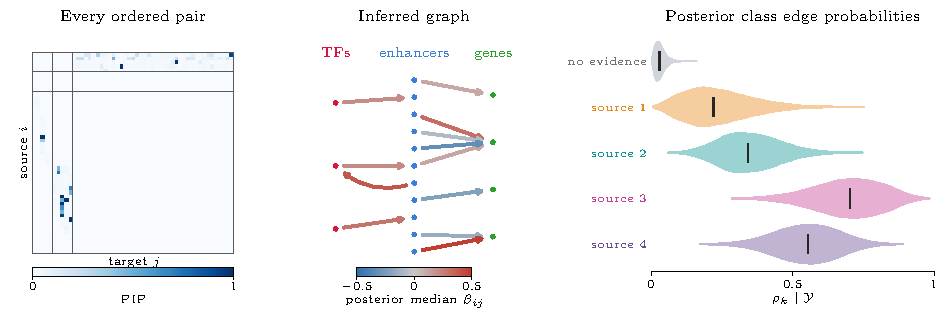
\includegraphics[width=15.9cm]{figures/fig1_panelG}};
\end{scope}
 \end{scope}

% model -> MCMC -> output
\draw[loop] (8.2,-9.45) -- (8.2,-9.72);
\draw[loop] (8.2,-11.35) -- (8.2,-11.62);

% What each band is, in a gutter to the left of the grid. The gutter sits outside
% the 16.4 cm the panels occupy rather than taking width from them: the figure is
% placed by \resizebox to a fixed fraction of \textwidth, so a wider drawing is
% scaled down rather than made to overflow, and none of the panels has to be
% re-laid-out to make room. Each band's extent is drawn as a rule beside its name.
\foreach \yt/\yb/\lab in {%
    0/-4.8/{Input},
    -5.1/-9.45/{Model},
    -9.75/-11.35/{Inference},
    -11.65/-18.0/{Output}}{
  \draw[black!20, line width=0.6pt] (-0.52,\yt) -- (-0.52,\yb);
  \node[band] at (-0.26,{0.5*(\yt+\yb)}) {\lab};
}

\end{tikzpicture}
